\section{Theoretical Analysis}
\label{sec:analysis}

\paragraph{} The values used in both analysis are the following:

$R_1$ = 1.00781211614 $k\Omega$
$R_2$ = 2.00311223204 $k\Omega$
$R_3$ = 3.04503555589 $k\Omega$
$R_4$ = 4.17896607062 $k\Omega$
$R_5$ = 3.10615699135 $k\Omega$
$R_6$ = 2.06090154363 $k\Omega$
$R_7$ = 1.00634569025 $k\Omega$
$V_s$ = 5.04864033546 V
$C$ = 1.02502620056 mA
$K_b$ = 7.05958243797 mS
$K_c$ = 8.03913881798 $m\Omega$

\subsection{Analysis for t<0}

\paragraph{} For t<0 we can see that we are working in the steady state, given that in that time interval $v_S$ = $V_S$. In a DC circuit, the capacitor charges up to it's full capacity, blocking the flow of electricity. Taking 
this into account we can replace the capacitor with an open circuit. With this information, and knowing that the the tension in $V_4$, since it is connected to ground, we can obtain the following equations.

\begin{equation}
\begin{bmatrix}
	-1	&	0	&	0	&	0	&	0	&	0	&	0 \\
	G_1	&	-G_1 - G_2 - G_3	&	G_2	&	G_3	&	0	&	0	&	0 \\
	0	&	-K_b - G_2	&	G_2	&	K_b	&	0	&	0	&	0 \\
	G_1	&	-G_1	&	0	&	-G_4	&	0	&	-G_6	&	0 \\
	0	&	0	&	0	&	0	&	0	&	G_6 + G_7	&	-G_7 \\
	0	&	0	&	0	&	-1	&	0	&	-G_6 *	K_d	&	1 \\
	0	&	G_3	&	0	&	-G_3 - G_4 - G_5	&	G_5	&	-G_6	&	0
\end{bmatrix}
\times
\begin{bmatrix}
	V_1 \\
	V_2 \\
	V_3 \\
	V_5 \\
	V_6 \\
	V_7 \\
	V_8
\end{bmatrix}
=
\begin{bmatrix}
	-V_s \\
	0 \\
	0 \\
	0 \\
	0 \\
	0 \\
	0
	\label{m:1}
\end{bmatrix}
\end{equation}

After solving them with the Octave sofware, we obtained the following results:

[INSERIR TABELA]

%\begin{table}[hbt!]
  %\centering
  %\begin{tabular}{|l|r|}
    %\hline    
 %   {\bf Name} & {\bf Value [mA]} \\ \hline
    %$I_{a}$ & -0.186554\\ \hline
$I_{b}$ & -0.195655\\ \hline
$I_{c}$ & 0.983196\\ \hline
$I_{d}$ & 1.025026\\ \hline

  %\end{tabular}
  %\caption{Mesh currents expressed in mA}
  %\label{tab:op}
%\end{table}

\subsection{Equivalent Resistance}

\paragraph{}In order to determine the equivalent resistance we need to determine $V_X$, this is, the difference between $V_6$ - $V_8$. This is made to ensure that the voltage in the capacitor is continuous.

Making use of the matrix below:

\begin{equation}
\begin{bmatrix}
	-1	&	0	&	0	&	0	&	0	&	0	&	0 \\
	G_1	&	-G_1 - G_2 - G_3	&	G_2	&	G_3	&	0	&	0	&	0 \\
	0	&	-K_b - G_2	&	G_2	&	K_b	&	0	&	0	&	0 \\
	G_1	&	-G_1	&	0	&	-G_4	&	0	&	-G_6	&	0 \\
	0	&	0	&	0	&	0	&	0	&	G_6 + G_7	&	-G_7 \\
	0	&	0	&	0	&	-1	&	0	&	-G_6 *	K_d	&	1 \\
	0	&	0	&	0	&	0	&	-1	&	0	&	1
\end{bmatrix}
\times
\begin{bmatrix}
	V_1 \\
	V_2 \\
	V_3 \\
	V_5 \\
	V_6 \\
	V_7 \\
	V_8
\end{bmatrix}
=
\begin{bmatrix}
	0 \\
	0 \\
	0 \\
	0 \\
	0 \\
	0 \\
	-V_x
	\label{m:1}
\end{bmatrix}
\end{equation}

And knowing that:

\begin{equation}
	V_x = V_6 - V_8
\end{equation}

\begin{equation}
	I_x = \frac{V_6 - V_5}{R_5} + \frac{V_3 - V_2}{R_2}
\end{equation}

\begin{equation}
	R_eq = \frac{V_x}{I_x}
\end{equation}

\begin{equation}
	\tau = R_eq * C
\end{equation}

We can obtain the following values:

[INSERIR TABELA]

\subsection{Natural Solution}

\paragraph{} The natural solution doesn't take into account idependent power sources. Using $V_x$ as the initial condition the natural solution can be obtained with the following equation

\begin{equation}
	V_{6n}(t) = V_x e^{(-\frac{t}{\tau})}
\end{equation}

After computing this data on Octave, we can plot the results of the interval [0, 20]ms.

\begin{figure}[!h]
	\centering
	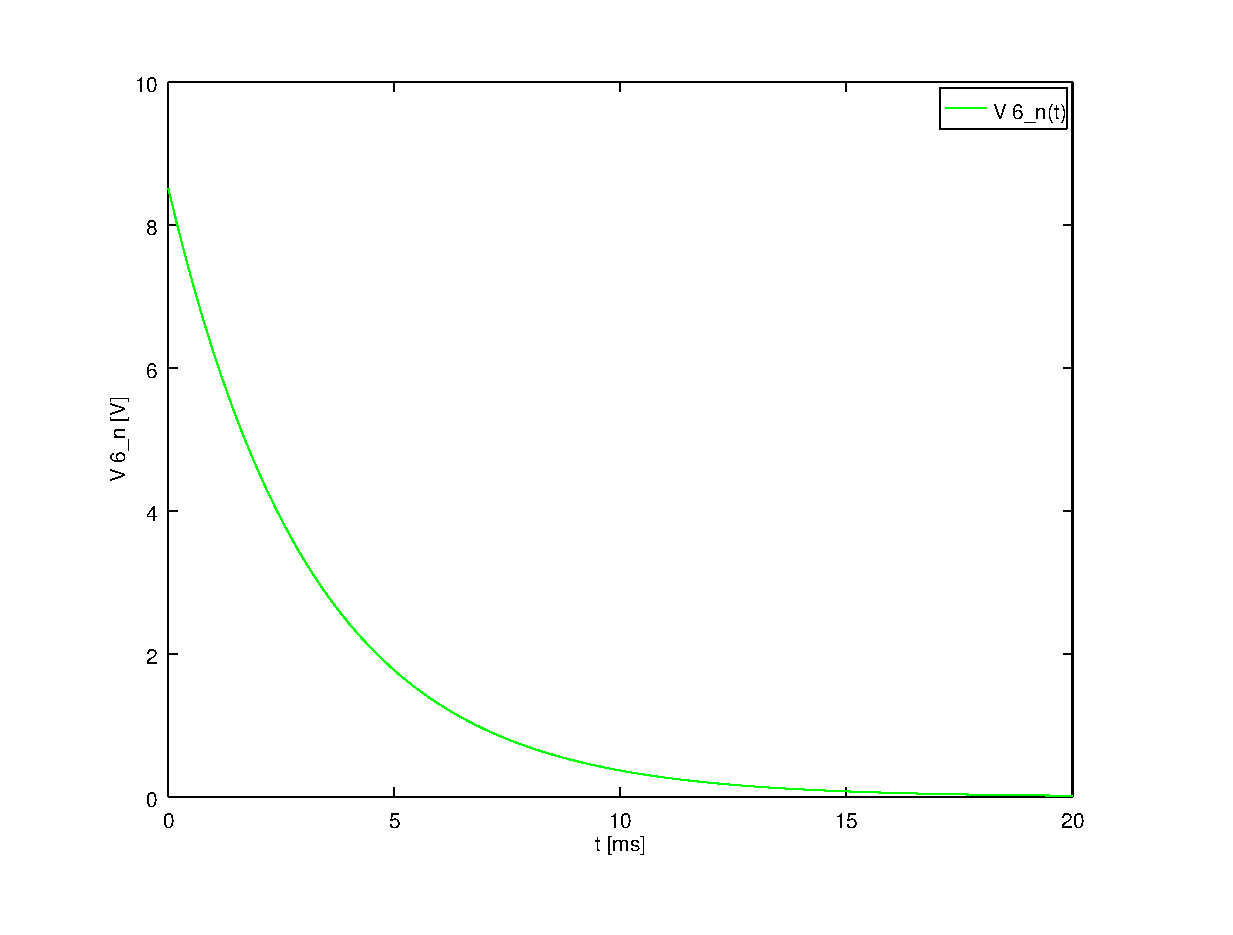
\includegraphics[width=0.7\linewidth]{natural.eps}
	\caption{Natural solution for t € [0, 20]}
\end{figure}

\subsection{Forced Solution}

\paragraph{} In order to obtain the forced solution we must be able to solve the following equation.  

\begin{equation}
\begin{bmatrix}
	-1	&	0	&	0	&	0	&	0	&	0	&	0 \\
	G_1	&	-G_1 - G_2 - G_3	&	G_2	&	G_3	&	0	&	0	&	0 \\
	0	&	-K_b - G_2	&	G_2	&	K_b	&	0	&	0	&	0 \\
	G_1	&	-G_1	&	0	&	-G_4	&	0	&	-G_6	&	0 \\
	0	&	0	&	0	&	0	&	0	&	G_6 + G_7	&	-G_7 \\
	0	&	0	&	0	&	-1	&	0	&	-G_6 *	K_d	&	1 \\
	0	&	G_3	&	0	&	-G_3 - G_4 - G_5	&	G_5 - jwC	&	-G_6	&	jwc
\end{bmatrix}
\times
\begin{bmatrix}
	V_1 \\
	V_2 \\
	V_3 \\
	V_5 \\
	V_6 \\
	V_7 \\
	V_8
\end{bmatrix}
=
\begin{bmatrix}
	-j \\
	0 \\
	0 \\
	0 \\
	0 \\
	0 \\
	0
	\label{m:1}
\end{bmatrix}
\end{equation}

From which we obtain the following values:

\begin{table}[hbt!]
  \centering
  \begin{tabular}{|l|r|}
    \hline    
    {\bf Name} & {\bf Value [mA]} \\ \hline
    $V_{1}$ & 1.000000 & -90.000000\\ \hline
$V_{2}$ & 0.947229 & -90.000000\\ \hline
$V_{3}$ & 0.832203 & -90.000000\\ \hline
$V_{5}$ & 0.955091 & -90.000000\\ \hline
$V_{6}$ & 0.551847 & 98.938374\\ \hline
$V_{7}$ & 0.360640 & 90.000000\\ \hline
$V_{8}$ & 0.549553 & 90.000000\\ \hline
  \end{tabular}
  \caption{Mesh currents expressed in mA}
  \label{tab:op}
\end{table}

\subsection{Final Total Solution}

\paragraph{} The final total solution is obtained by superimposing both natural and forced responses:

\begin{equation}
	V_6(t) = V_{6f}(t) + V_{6n}(t)
\end{equation}

We can see the plot of $V_s(t)$ and $V_6(t)$ from -5ms to 20ms [Observações].

\subsection{Frequency Response}

We can see that for low frequencies (<1Hz) every voltage is in phase. The capacitor is given enough time to charge up to the same voltage 
as the voltage source.

\begin{figure}[!h]
	\centering
	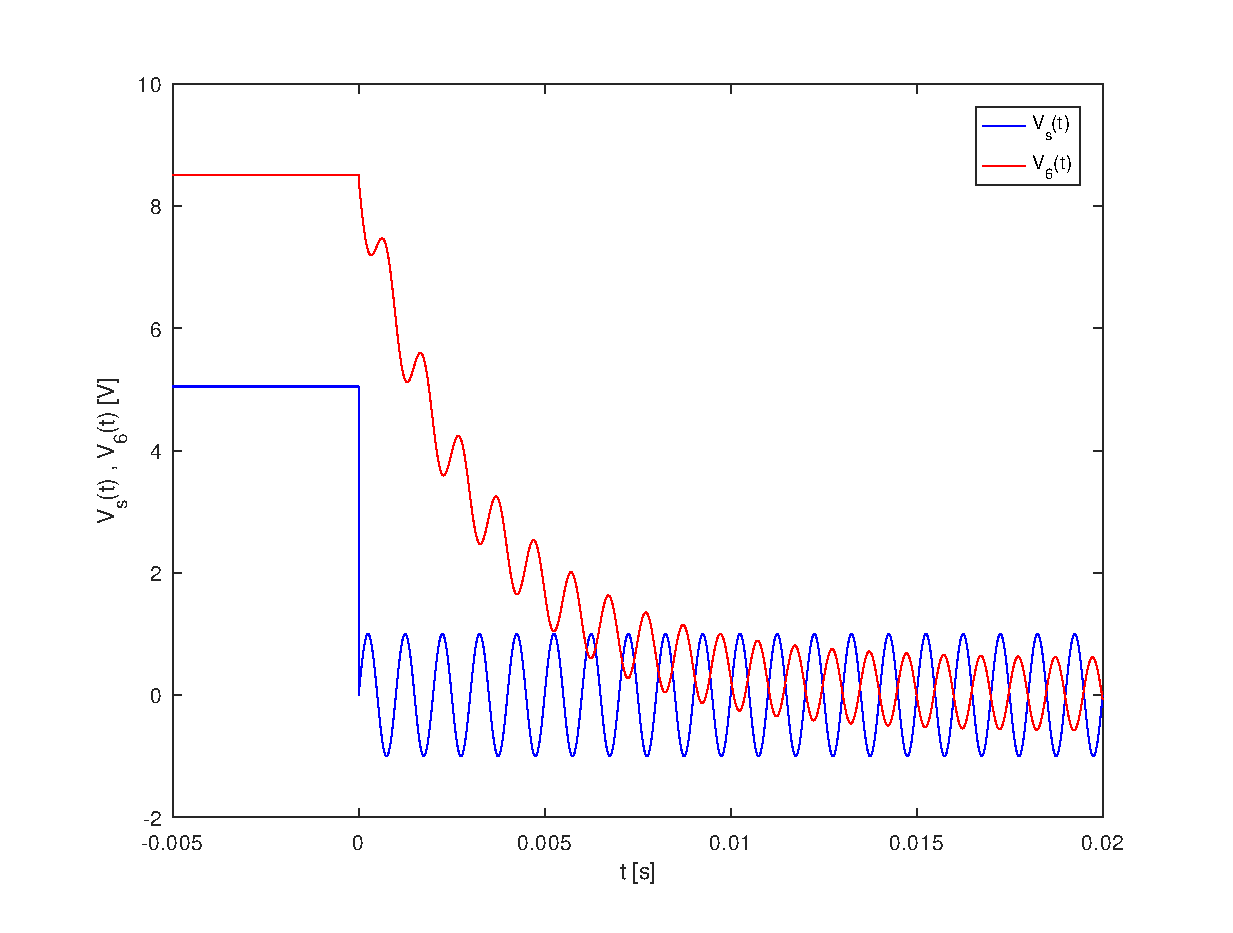
\includegraphics[width=0.7\linewidth]{total.eps}
	\caption{Total solution for $V_6$ and $V_s$}
\end{figure}

\begin{figure}[!h]
	\centering
	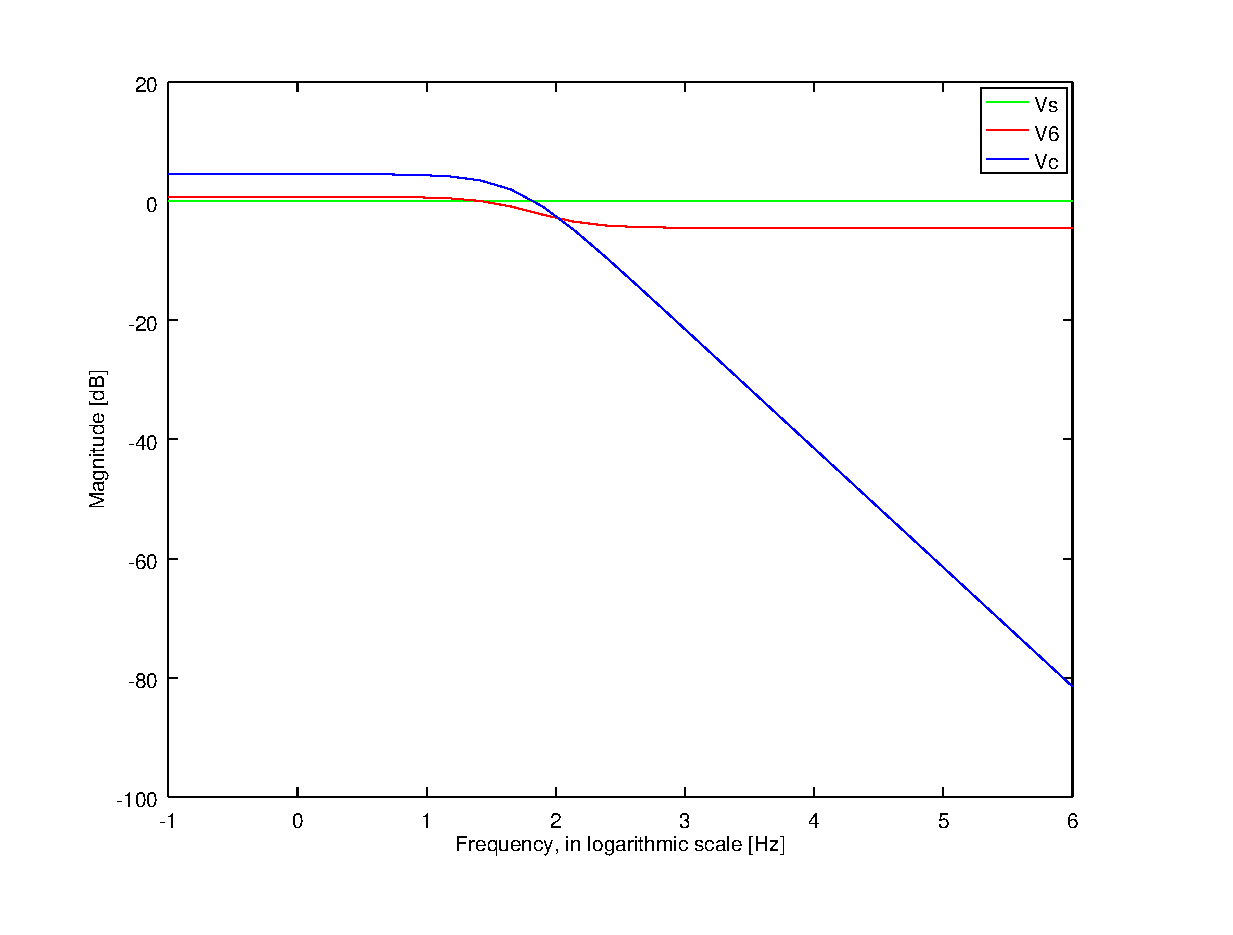
\includegraphics[width=0.7\linewidth]{magnitude.eps}
	\caption{Variation of frequency of $V_s$, $V_6$ and $V_c$ voltage magnitudes}
\end{figure}

\begin{figure}[!h]
	\centering
	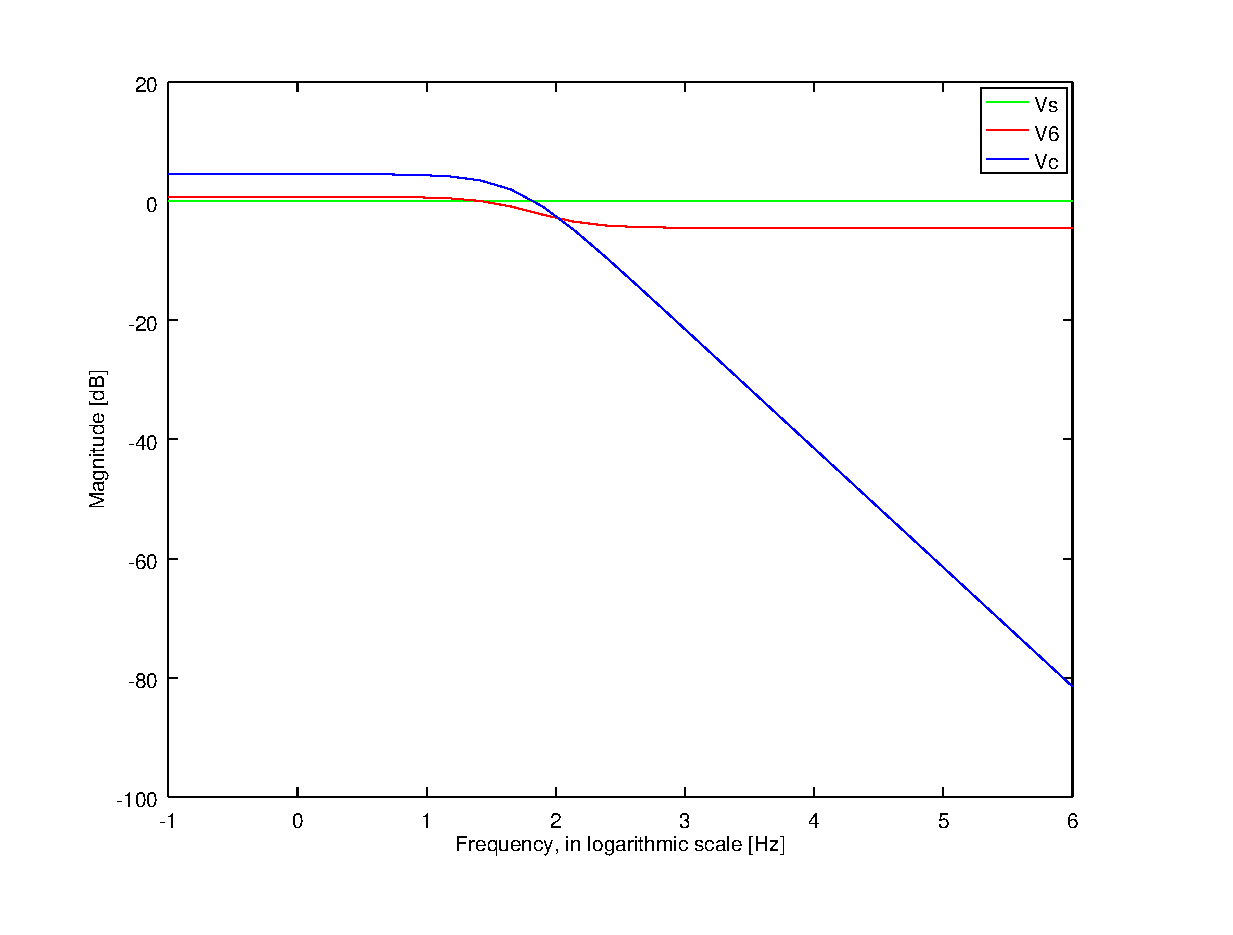
\includegraphics[width=0.7\linewidth]{magnitude.eps}
	\caption{Variation of frequency of $V_s$, $V_6$ and $V_c$ voltage phases}
\end{figure}



